\section{Exercise 1 - Mid-depth temperature and \delO{SW} reconstruction}

\subsection{Question 1}
\label{sec:Q1}
According to \citeauthor{barker2003study} \parencite{barker2003study}, foraminiferal Fe/Mg molar ratios greater than approximately 0.1 are indicative of potential contamination by Mg-rich clay silicates.
Mg/Ca measurements could therefore be rejected if they do not meet the criteria:

\begin{equation} \label{eq:fe_mg}
    \frac{\mathrm{Fe}/\mathrm{Ca}}{\mathrm{Mg}/\mathrm{Ca}} < 0.1 \, \mathrm{mol \cdot mol^{-1}}
\end{equation}

However, visual assessment of the magnitude of potential contamination (Figure \ref{fig:Mg_Fe}) shows that all but one of the eight measurements failing the this criteria are close to the rest of the data in terms of Fe/Mg.
As a result, only the 16.39 ka measurement labelled in Figure \ref{fig:Mg_Fe} is rejected for contamination.

\begin{figure}[h!]
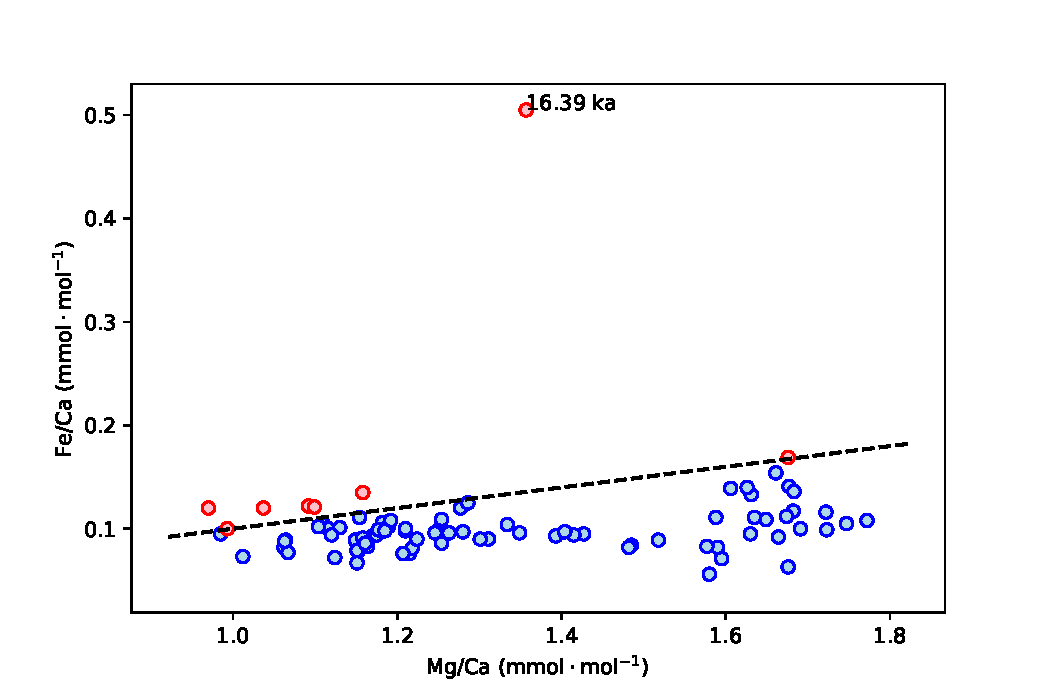
\includegraphics[width=\textwidth]{img/scatter_MgCa_x_FeCa_contaminated.pdf}
    \caption{Ratio of Mg/Ca to Fe/Ca in benthic foraminifera \emph{M. barleeanuum} in intermediate sediment core RAPiD-10-1P, on the South Iceland Rise.
             Dashed line seperates potentially contaminated measurements (red points) according to Equation \ref{eq:fe_mg}.
             Labelled point is identified for rejection.}
        \label{fig:Mg_Fe}
\end{figure}

\subsection{Question 2}
As shown in Figure \ref{eq:timeseries}, the mid-depth seawater oxygen isotope excursion \delO{SW} declines to negative values after the Last Glacial Maximum (LGM) in correspondance with falling water temperatures.
The two trends fall sharply toward the beginning of Heinrich Stadial 1 (HS1) before diverging: in contrast to the gradual temperature recovery from nearly 0 \degree{}C, \delO{SW} continues to strongly decrease until the transition into the Bølling–Allerød warm period (BA, 14.7–12.9 ka \parencite{thornalley2011reconstructing}), at which point both lines rise together rapidly.
The Younger Dryas (YD) marks a very abrupt return to HS1 temperatures, although the concurrent drop in \delO{SW} is not as severe, whereas each record shows relative stability over the course of the Holocene.

The imprint of local salinity on foramineferal Mg/Ca may result in significant systematic positive bias in reconstructed \delO{SW} \parencite{mathien2009salinity}, whereas uncertainties in foramineferal \delO{carbonate} stemming from nonclimatic factors, such as measurement imprecision or variations in seawater carbonate ion concentration, are comparatively small \parencite{bell2014local}. 
Assuming these issues are negligeable, the control of water oxygen isotopic composition hydrological fractionation processes at the surface make it useful proxy for salinity, from which an interior ocean water mass's surface origin can be inferred \parencite{ravelo2007use, lynch2014tracers}.
Although sea ice formation may be an important control on intermediate water salinity, given the subpolar location of the RAPiD-10-1P core, the relatively small isotopic effect of brine rejection means that the surface source \delO{SW} signal is largely unaltered \parencite{waelbroeck2011timing}. 
Therefore, in accordance with similiar studies \parencite[e.g.][]{thornalley2010intermediate, thornalley2011reconstructing}, the changes in \delO{SW} and Temperature over HS1 (Figure \ref{eq:timeseries}) could be interpreted to show the displacement of cold, hypersaline, \delO{}-enriched polar waters, originating from open-ocean convection, by an increasing sink of warmer, isotopically lighter glacial meltwater due to enhancement of local brine formation, while the abrupt drops preceeding HS1 appear to record large-scale freshening events.
These results support previous studies hypothesising the suppression of traditional North Atlantic Deep Water (NADW) during deglacial stadials by intense ocean stratification associated with the massive input of freshwater into the North Atlantic from the Northern Hemispheric ice sheets \parencite{vidal1998benthic, dokken1999rapid}.

\begin{figure} \label{eq:timeseries}
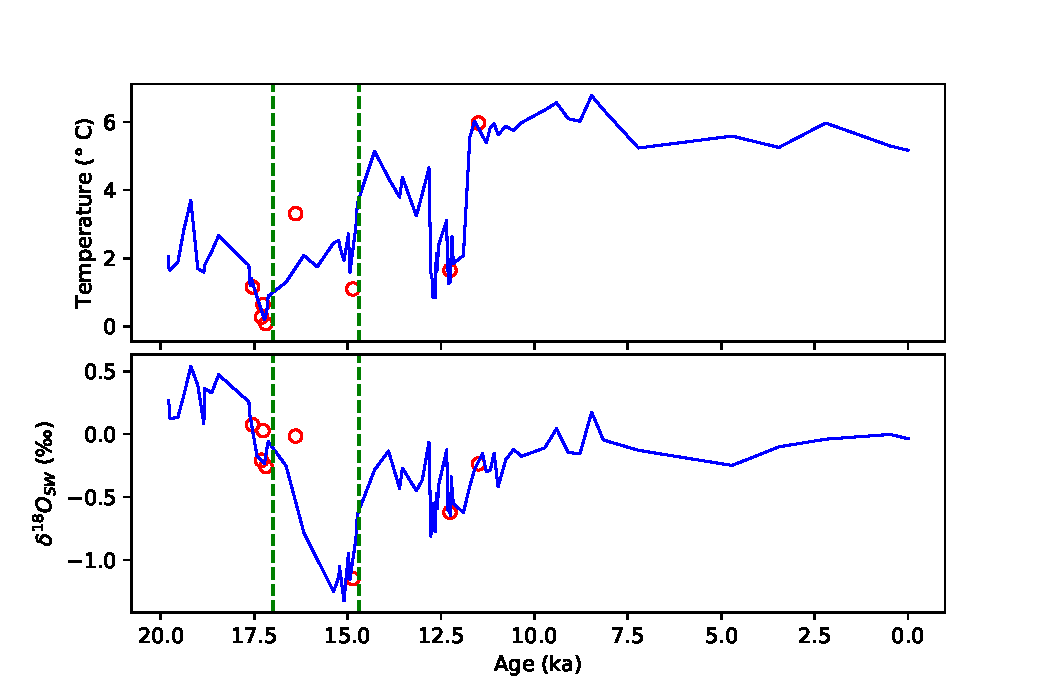
\includegraphics[width=\textwidth]{img/timeseries_temp_and_d18Osw.pdf}
    \caption{Trends in the ice-volume corrected \delO{SW} (top) and mid-depth water temperature since the Last Glacial Maximum determined from Mg/Ca palaeothermetry (bottom) recorded in RAPid-10-1P.
             Red points and the gap in the timeseries signify a rejected measurement (see text in Section \ref{sec:Q1}).
             Shaded regions mark Heinrich Stadial 1 (HS1) and Younger Dryas (YD), as defined in \citeauthor{thornalley2011reconstructing} \parencite{thornalley2011reconstructing}.}
        \label{fig:timeseriestempd18Osw}
\end{figure}
